\chapter{Experiment \& Result}
This chapter explains experiment setup and showing the result for all process from the proposed method in the chapter 4. In additional, each process has to full fill its own objectives as well as satisfy the objective of this thesis overall. 
\section{Dataset}
All dataset in our experiment are collected in an open area with no obstacle between tracker and receiver inside the 6th floor of the International College building in King Mongkut’s Institute of Technology Ladkrabang (KMITL) at eight different angle of rotations of the tracker: angle 0, angle 45, angle 90, angle 135, angle 180, angle 225, angle 270, and angle 315.\\
\\
\noindent \textbf{Training Sets}
\newline Following is the list of all datasets we collected using Raspberry Pi 3 Receive and BLE tracker.
\begin{enumerate}
    \item Dataset 1: 200 samples at 12 distances, 0.5, 1, 1.5, 2, 2.5, 3, 3.5, 4, 4.5, 5, 5.5, and 6 meters collected on October 17, 2018.
    \item Dataset 2: 200 samples at 12 distances, 0.5, 1, 1.5, 2, 2.5, 3, 3.5, 4, 4.5, 5, 5.5, and 6 meters collected on November 12, 2018.
    \item Dataset 3: 200 samples at 12 distances, 0.5, 1, 1.5, 2, 2.5, 3, 3.5, 4, 4.5, 5, 5.5, and 6 meters collected on November 21, 2018.
    \item Dataset 4: 200 samples at 12 distances, 0.5, 1, 1.5, 2, 2.5, 3, 3.5, 4, 4.5, 5, 5.5, and 6 meters collected on December 04, 2018.
    \item Dataset 5: 200 samples at 12 distances, 0.5, 1, 1.5, 2, 2.5, 3, 3.5, 4, 4.5, 5, 5.5, and 6 meters collected on February 20, 2019.
    \item Dataset 6: 200 samples at 12 distances, 0.5, 1, 1.5, 2, 2.5, 3, 3.5, 4, 4.5, 5, 5.5, and 6 meters collected on March 1, 2019.
\end{enumerate}
\section{Measure}
\subsection{Root Mean Squared Eror(RMSE)}
The statistical measures that we use to evaluate the performance of our
system are the minimum absolute error, maximum absolute error, standard deviation of the absolute errors and the Root Mean Squared Error (RMSE). The
absolute error measures the absolute difference between the expected and the
actual result. RMSE basically measures the average of the differences between
the expected and the actual results, calculated by Eq \ref{RMSE}
\begin{equation}
RMSE = \sqrt{\frac{1}{n} \sum_{i=1}^{n} (y_i-\hat{y_i})^2}
\label{RMSE}
\end{equation}
where $n$ is the number of predictions, $y$ is the vector of expected values and $\hat{y}$ is the vector of actual values being predicted.
\subsection{Precision Score}
The precision score is ratio of correctness,it is a metric for multi-label classification of how many selected items are relevant
\begin{equation}
Precision Score = \frac{TP}{TP+FP}
\label{precision}
\end{equation}
where $tp$ is the number of true positives and $fp$ the number of false positives. The precision is intuitively the ability of the classifier not to label as positive a sample that is negative.
The best value is 1 and the worst value is 0.


\section{Experiment}
There are four experiments on all of our datasets to study the nature of the data and formulate hypotheses. In this section, the author explore the factors that related to the performance of the system. It consist of Preprocessing technique, and environment variable in Path loss model. 
\subsection{Experiment1: Preprocessing by Moving Average}
\subsection*{Objective}
\noindent This experiment explains the effectiveness of RSSI after reducing the noise of data by using moving average and visualize the path loss model from the moving average of RSSI data.


\subsection*{Experimental Procedure}
The raw RSSI set is filtered by moving average with a windows size of 20, using Matlab on test set for all 8 angles of vertical rotation to smooth the RSSI readings before the curve fitting is performed on the means of the filtered data to obtain the
path loss model

\begin{figure}[H]
\centering
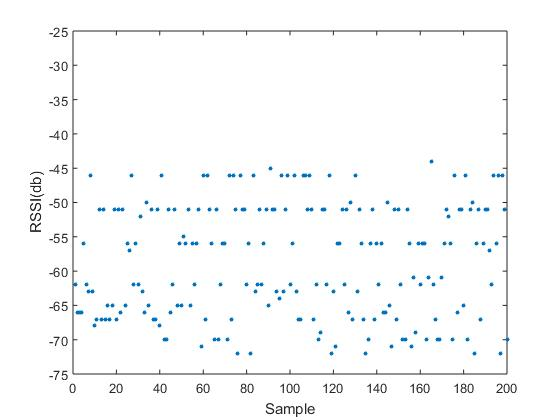
\includegraphics[width=\textwidth]{Image/scatterRaw.jpg}
\caption{Scatter plot of raw data}
\label{}
\end{figure}


\begin{figure}[H]
\centering
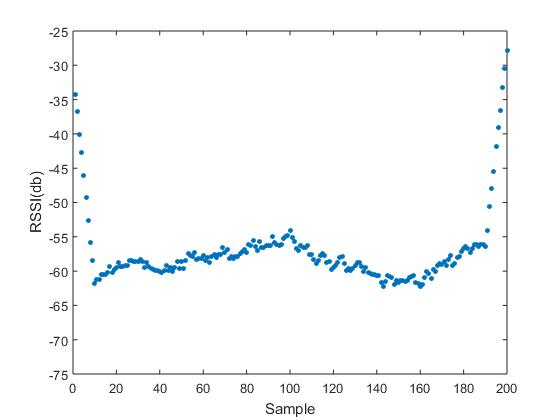
\includegraphics[width=\textwidth]{Image/s05Avg.jpg}
\caption{Scatter plot of data after applying moving average}
\label{}
\end{figure}



\subsection*{Result}
The data is less scatter and smoother after applying the moving average. The data before applying the moving average is shown in Fig.6.1 and the data after applying the moving average is shown in Fig.6.2.

\begin{figure}[H]
\centering
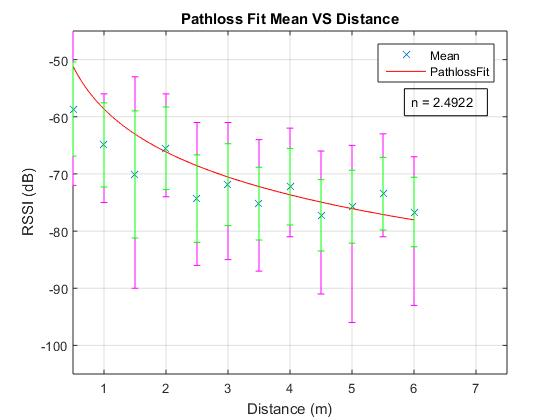
\includegraphics[width=\textwidth]{Image/rawCurveFit0.jpg}
\caption{Curve fitting of raw data at angle 0}
\label{}
\end{figure}

Fig.6.3 shows the result of curve fitting to pathloss model of raw data at angle 0. The pink bar at each point indicates its min-max error bar, while the green bar indicates its standard deviation.

\begin{figure}[H]
\centering
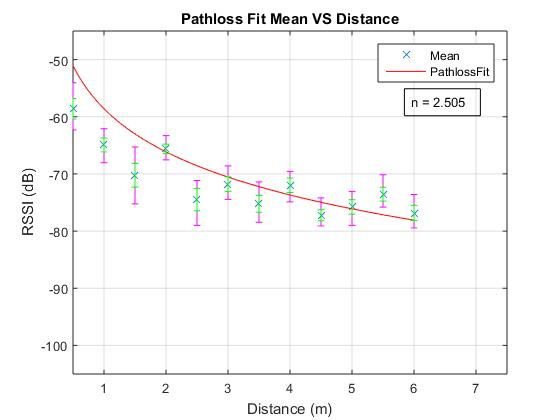
\includegraphics[width=\textwidth]{Image/curveFit0.jpg}
\caption{Curve fitting of data at angle 0 after applying moving average}
\label{}
\end{figure}

Fig.6.4 shows the result of curve fitting to pathloss model of the data at angle 0 after filtering with moving average. From the observation, the min-max error bar and the standard deviation in Fig.6.4 is significantly smaller comparing to the plot shown in Fig.6.3. The conclusion of statistics from before applying filter and after applying filter is shown in Fig.6.5 and Fig.6.6 respectively.

\begin{figure}[H]
\centering
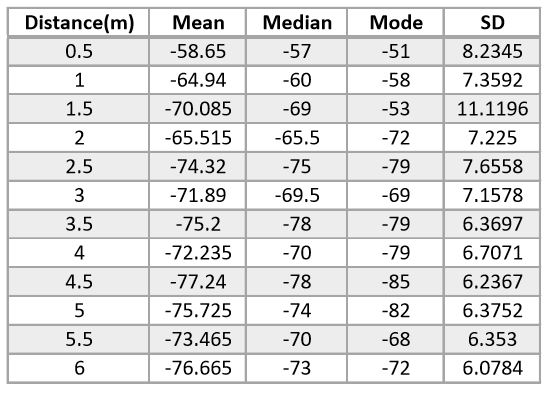
\includegraphics[width=\textwidth]{Image/rawTable.JPG}
\caption{Statistics details of raw data at angle 0}
\label{}
\end{figure}

\begin{figure}[H]
\centering
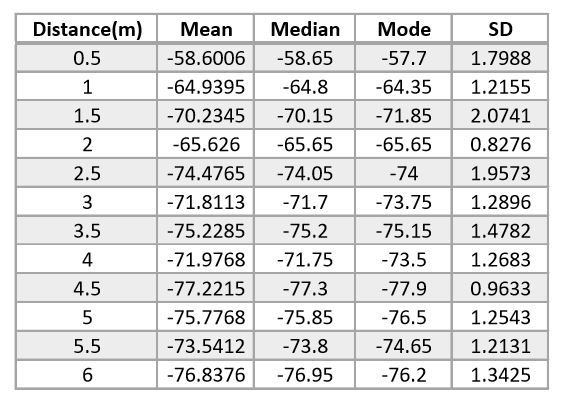
\includegraphics[width=\textwidth]{Image/movAvgTable.JPG}
\caption{Statistics of data at angle 0 after applying moving average filter}
\label{}
\end{figure}



\subsection{Experiment2: Prediction of $n$ variable in Path Loss Model}
\subsection*{Objective}
This experiment is conducted in an attempt to predict the $n$ variable which is the environment variable that can directly affect to the accuracy of RSSI-Distance Conversion (Distance Estimation) in Eq. (4.4)
\subsection*{Experimental Procedure}
The curve fitting to pathloss model is performed on filtered RSSI data. After the curve fitting process and the $n$ variable is obtained, we to plot the value of $n$ from we retrieved from curve fitting at every angles and observe the trend of the graph.

\begin{figure}[H]
\centering
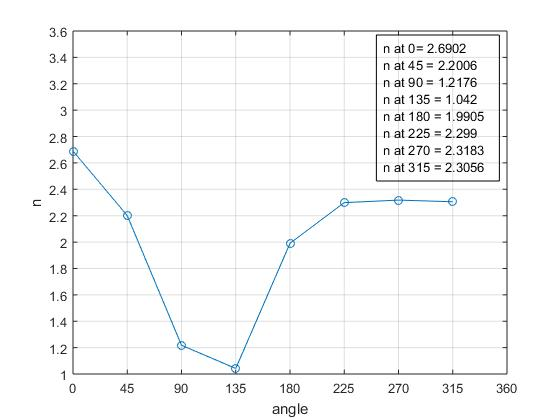
\includegraphics[width=\textwidth]{Image/pltN1.jpg}
\caption{Plot of $n$ from Dataset 1}
\label{}
\end{figure}

\begin{figure}[H]
\centering
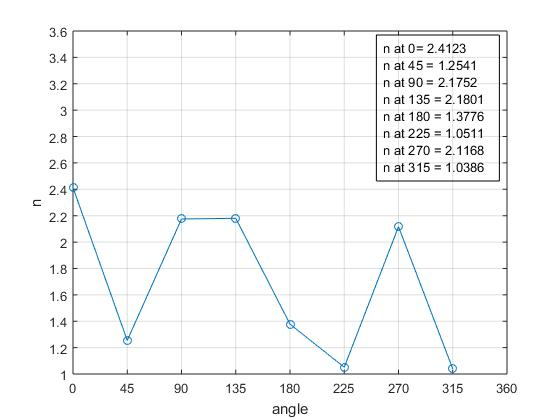
\includegraphics[width=\textwidth]{Image/pltN2.jpg}
\caption{Plot of $n$ values from Dataset 2}
\label{}
\end{figure}

\begin{figure}[H]
\centering
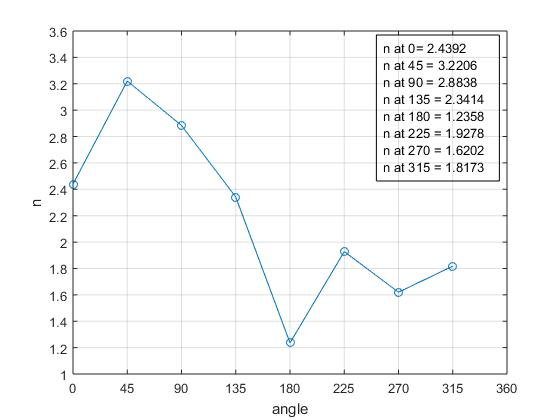
\includegraphics[width=\textwidth]{Image/pltN3.jpg}
\caption{Plot of $n$ values from Dataset 3}
\label{}
\end{figure}

\begin{figure}[H]
\centering
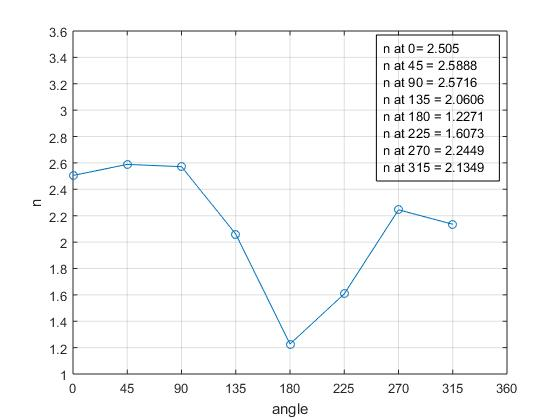
\includegraphics[width=\textwidth]{Image/pltN4.jpg}
\caption{Plot of $n$ values from Dataset 4}
\label{}
\end{figure}

\subsection*{Result}
We did this experiment in hope to be able to determine the pattern of the graph by observing each plot. However, unfortunately, the pattern that we get from each dataset varies too much to be able to infer the overall pattern. For example, the pattern from Fig.6.8 is similar to the graph of sine, though, the same cannot be said for the rest. The pattern from Fig.6.9 and Fig.6.10 is similar to each other as their RSSI data were collected on the same date and almost at the same time. Nevertheless, there is an inadequate information to conclude the pattern according to the graph trend.

\subsection{Experiment 3: Trilateration}
\subsection*{Objective}
This experiment is conducted to evaluate the performance of trilateration by the
path loss models of known angle (angle 0) obtained from preprocessing techniques: moving average with window size of 20
separation technique
\subsection*{Experimental Procedure}
Our training set consists of the RSSI data of angle 0 from Dataset 5.
It is preprocessed by applying a moving average filter and then curve fitted
to obtain the pathloss models. 

For the test set, we use the 200 samples of RSSI data that are collected real-time
by each receiver. Similar to the training set, it is preprocessed by applying the 
moving average filter and curve fitted into the pathloss models to estimate
the distance between the target object and the receiver before applying the trilateration
technique to acquire the position of the target object. The three closest
receivers based on the distance between receiver and tracker(target object) will be
used for the trilateration. Figure \ref{fig:tri_setup} and \ref{fig:realtri_setup} show the setup of receiver and tracker
for the trilateration experiment.

\begin{figure}
\centering
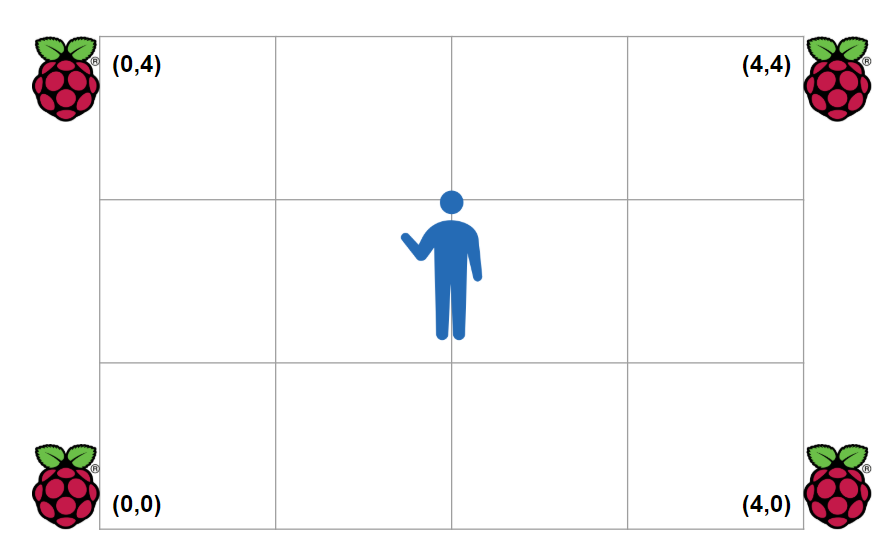
\includegraphics[width=\textwidth]{Image/area.png}
\caption{Overview of Trilateration Setup}
\label{fig:tri_setup}
\end{figure}

\begin{figure}
\centering
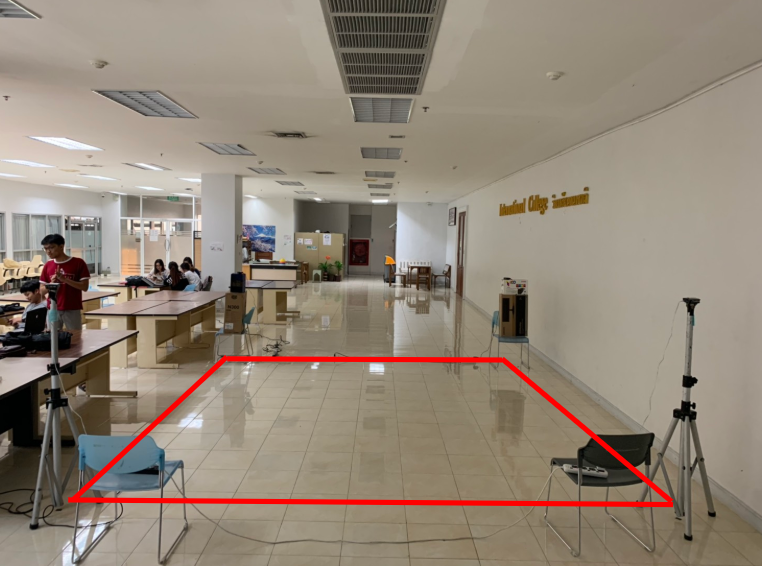
\includegraphics[width=\textwidth]{Image/realarea.png}
\caption{Trilateration Setup on 6th Floor of IC KMTL }
\label{fig:realtri_setup}
\end{figure}

\newpage
\subsection*{Result}
From the table, it show the performance comparison of trilateration at different position based on Root Mean Square Error(RMSE), minimum absolute error, maximum absolute error and the standard deviation (SD) of the absolute errors. In RMSE the value that close to 0 that mean no error occur. However, it can see that the minimum and maximum, of RMSE are 0.62 and 1.19 respectively, it can conclude that are very high RMSE and illustrate there are a huge error on this experiment.
\begin{table}[]
\begin{tabular}{|l|l|l|l|l|l|l|}
\hline
                           & \multicolumn{1}{c|}{(0,0)} & \multicolumn{1}{c|}{(1,0)} & (2,1) & (3,3) & (0,4) & (4,4) \\ \hline
\multicolumn{1}{|c|}{RMSE} & 0.86                       & 1.19                       & 0.62  & 0.82  & 0.83  & 1.1   \\ \hline
Min Abs Error              & 0.14                       & 0.04                       & 0.48  & 0.16  & 0.13  & 0.14  \\ \hline
Max Abs Error              & 2.40                       & 2.6                        & 3.1   & 2.56  & 1.7   & 4.25  \\ \hline
\multicolumn{1}{|c|}{SD}   & 0.71                       & 0.77                       & 0.89  & 0.64  & 0.52  & 1.16  \\ \hline
\end{tabular}
\caption{Statistics of trilateration result}
\label{result_rmse}
\end{table}

\newpage
\subsection{Experiment 4: Trilateration with logic condition}
\subsection*{Objective}
This experiment tired to reduce the error in RMSE from Experiment 3 by setting logic condition rule to avoid the fluctuate result which product from tracker
\subsection*{Experimental Procedure}
Due to the high error of RMSE that show in Experiment 3, this experiment tried to reduce error by making logic condition. From \ref{diagram_logic}, it can be obviously seen that after trilateration computing to get the coordinate position of object ex (1,3), it will sent this value to logic condition process to compute. After that,system will get the result. Figure \ref{logicalgo} it demonstrate the result from logic condition when position of object is inside the range of that are set. For instance, if the position of object is (1,1.5) after pass to logic condition, the result will be "Block1"

\begin{figure}[h]
\centering
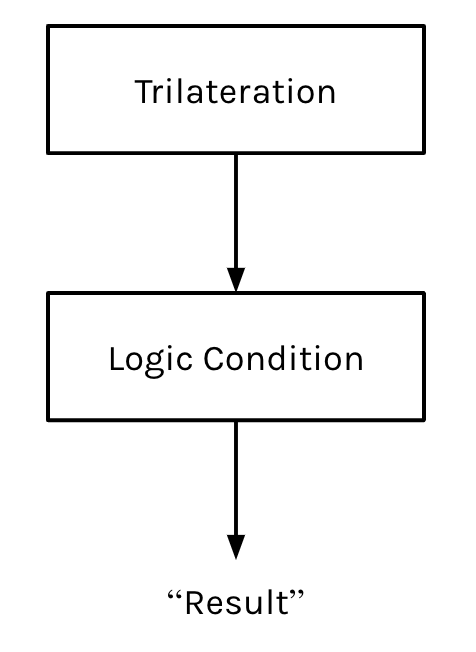
\includegraphics[width={0.4\textwidth}]{Image/diagram_logic2.png}
\caption{}
\label{diagram_logic}
\end{figure}

\begin{figure}[h]
\centering
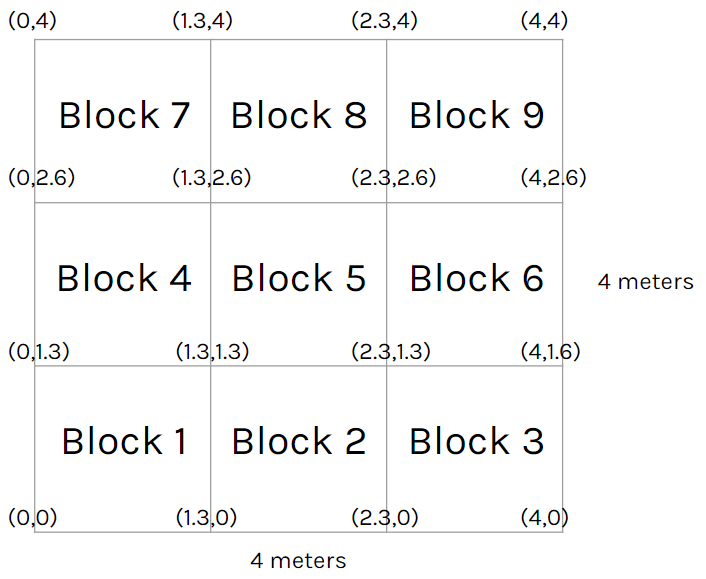
\includegraphics[width={\textwidth}]{Image/blog33.png}
\caption{}
\label{logicalgo}
\end{figure}



\newpage
\subsection{Result}
From table \ref{result_rmse2}, it show the precision score of trilateration with logic condition,the highest precision score is 0.88 at block9 and lowest score is 0.77. Moreover, the standard deviation is 0.053 that means that the result do not have a lot of “spread”. The result in the sample don't vary much, and are very tightly clustered together.
\newline
\begin{sidewaystable}[]
\begin{tabular}{|l|l|l|l|l|l|l|l|l|l|}
\hline
                                                                                         & Block1 & Block2 & Block3 & Block4 & Block5 & Block6 & Block7 & Block8 & Block9 \\ \hline
Precision Score                                                                          & 0.91   & 0.69   & 0.91   & 0.60   & 0.47   & 0.65   & 0.91   & 0.52   & 0.91   \\ \hline
\multicolumn{1}{|c|}{\begin{tabular}[c]{@{}c@{}}Average \\ Precision Score\end{tabular}} & \multicolumn{9}{c|}{0.73}                                                     \\ \hline
\multicolumn{1}{|c|}{SD}                                                                 & \multicolumn{9}{c|}{0.17}                                                     \\ \hline
\end{tabular}

\caption{Statistics of trilateration with logic condition result}
\label{result_rmse2}
\end{sidewaystable}
